%!TEX root = ../thesis.tex

\chapter{Introduction}
\label{chap:intro}

\section{Motivation}
\label{sec:motivation}

\Gls{it} is constantly shaping the world that we live in. The advancements in \gls{it} has changed the patterns of human behavior and influenced the way we connect with our environment. The ease with which digital content is generated and shared, further propels the growth of these technologies. Music being a universal socio-cultural phenomena has been deeply influenced by these advancements. The way music is created, stored, disseminated, listened, and even learnt has undergone severe changes. A massive amount of audio music content is now available on demand. In order to facilitate interaction with such large volumes of digital music content It becomes necessary to develop computational techniques that can automatically describe and deal with this digital music content in a meaningful way. There can be different information sources such as editorial metadata, social data, and audio recordings that can be exploited to generate a description of music. In this thesis we focus on the audio music content, which is also referred as music content processing. 

Melody is a fundamental music dimension, along with harmony and rhythm, and thus, an indespensible component in the description of music. As put by (Selfridge-Field, 1998). 

It is melody that enables us to distinguish one work from another. It is melody that human beings are innately able to reproduce by singing, humming, and whistling. It is melody that makes music memorable: we are likely to recall a tune long after we have forgotten its text. 

The importance of melody in our musical experiences makes its analysis and description a crucial component in music content processing.  It becomes even more important for melody dominant music traditions such as IAM, where the concept of harmony from a music point of view does not exist, and the complex melodic structure takes the central role in music aesthetics.

Melodic analysis and description is not a recent phenomenon, it has been manually done by musicologists for hundreds of years (REF). However, a computational approach to this task has opened up new directions and possibilities, giving such an analysis a different magnitude altogether. Through computational approaches such analyses can be applied at the level of an entire music repertoire, as opposed to a few music pieces typically considered in manually performed musicological studies. Of course, computational melodic analysis is a work in progress and there are constant attempts to generate a meaningful description that resembles closely to what can be done by human experts.

Current computational approaches for describing melodies primarily work with symbolic representations of music, which only cover a particular view of music. There are significant challenges in extending such approaches to analyze recorded performances, mainly due to the difficulties involved in obtaining a meaningful symbolic representation from audio recordings. Therefore, for performance oriented music traditions such as IAM, where the aesthetics lie mainly in the improvisatory aspects of the music, and symbolic music representations are practically nonexistent, such approaches are not directly applicable. Besides, melody, being a cultural phenomenon, should be studied within the cultural context of a music tradition. Thus, we need culture-aware approaches that can utilize specific melodic characteristics of music traditions to generate its meaningful melodic description.

Indian art music with its complex melodic framework, \gls{raga}, and well grounded-music theory provides an interesting context to develop computational approaches for melodic description of recorded music performances. Different melodic elements in IAM are hierarchically organized in accordance with the raga grammar. At the lowest level there are \glspl{svara}, which concatenate to form melodic phrases. These phrases group together to form passages, and finally leading to a music piece. In this thesis we focus on computational approaches that analyse these melodic elements at different hierarchical levels to describe melodic aspects of music collections in IAM. Furthermore, performing an analysis at the level of an entire music collection allows us to relate these melodic elements across recordings and study corpora level melodic aspects. YAAR PLS ACCHE SE LIKHWA DO!! 

Analysis and description of melodies elements mentioned above is a useful task with manifold applications. Such an analysis can enable corpora level musicological studies such as characterization of different compositions, artists and ragas in audio music collections. Since IAM follows an oral pedagogy, such an analysis of the recorded performances can shed lights on the stylistic influences of a teachers on their students, or across artists in general. Analyzing and relating different melodic elements in a music collection opens up ways to define novel music similarity measures, and generate semantically meaningful description of higher level musical concepts such as ragas. This in turn enables several applications such as structuring and organizing of large music collections, raga-based music retrieval and musically relevant music navigation and discovery. A rich description of differnet melodic elements also aids in novel applications addressing enhanced or augmented music listening experience. This aspect specifically relevant in IAM where the music is said to be accessible mainly to musicians and  connoisseurs owing to the complexity of the melodic structures. Besides this, able to analyse and characterize different melodic elements directly from audio recordings opens up novel and creative ways to approach music pedagogy. Specially in the context of IAM where the nuances of the music are learned implicitly through years of training, where analytical and objective description of music performances is largely nonexistent, an objective melodic description can aid music students to learn from the recorded performances of Mastros. 

\section{Scientific Context and Relevance}
\label{sec:context}

\Gls{mir} is a growing interdisciplinary research field that stands at the intersection of well established disciplines such as signal processing, pattern recognition, musicology, psychoacoustics, music perception and cognition, information science, and computer science (machine-learning). \Gls{mir} primarily addresses topics involved in the understanding and modeling of music using information processing methodologies~\citep{roadmap_mir}. In particular, it aims to advance our knowledge in representing, understanding, describing, retrieving, archiving and organizing music related data. This opens up a wealth of possibilities to develop novel ways to interact with music~\citep{casey2008content,orio2006music,burgoyne2016music}.  

The field of \gls{mir} has made significant advancements in the last two decades. Its growth is fueled by the massive surge in the digital music content. However, many of the technologies developed within \gls{mir} are not directly applicable to several music cultures of the world. This can be largely attributed to the fact that the research in \gls{mir} has been mainly focused on the western commercial music of the past few decades~\citep{XavierSerra2011}, which has largely shaped the research problems undertaken in \gls{mir}. A significant effort in \gls{mir} is dedicated towards automatic description and characterization of music content to extract musically and semantically relevant information. Computational approaches in \gls{mir} address a variety of tasks such as melody extraction~\citep{salamon:phd:13}, chord estimation~\citep{mcvicar2014automatic}, music key estimation~\citep{peeters2006chroma}, motif discovery~\citep{collins2011improved,Conklin2010}, music structure analysis~\citep{paulus2010state,serra2012unsupervised}, music similarity~\citep{joan_thesis}, genre classification~\cite{aucouturier2003representing} and emotion recognition~\citep{kim2010music}, tempo and beat tracking~\citep{gouyon2005review,scheirer1998tempo}. These approaches describe and characterize music recordings in terms of different musical aspects such as melody, rhythm, harmony, structure and emotion. The definition, interpretation and relevance of these musical aspects are not universal and vary significantly across different music traditions,  and personal, cultural and social contexts. However, a significant number of existing computational approaches in \gls{mir} fail to account for these factors, and thus, might be hitting the so-called ``glass ceiling"~\citep{pachet2004improving,casey2008content}. This phenomenon is evident from the slowing rate of improvement in the approaches in \gls{mir} over years, as seen in the results of MIREX\footnote{http://www.music-ir.org/mirex/wiki/MIREX\_HOME} evaluations. There also exists a semantic-gap between the automatically extracted music descriptors from audio signals and the high level music concepts that humans relate to~\citep{celma2006foafing,casey2008content}. There is a need to bridge this gap and take a broader perspective to describe music by taking the cultural, social and user context into account~\citep{roadmap_mir}. It is in this context that the CompMusic project was envisioned~\citep{XavierSerra2011}.

CompMusic\footnote{http://compmusic.upf.edu/} (Computational Models for the Discovery of the World'd Music) is a research project funded by the European Research Council. The project focuses on five music traditions of the world: Hindustani (North India), Carnatic (South India), Turkish-makam (Turkey), Arab-Andalusian (Maghreb), and Beijing Opera (China). One of the main objectives of the CompMusic project is to promote and develop multicultural perspectives in \gls{mir}. In particular, the project aims to advance the research in computational description of music by identifying musically relevant problems coming from culture-specific contexts and developing domain specific approaches to solve them. Addressing the research problems in the context of diverse music cultures will not only help in advancing the knowledge in the specific cultures, but also expand the scope of current research in \gls{mir}. Furthermore, it can help bridge the semantic-gap and push the glass-ceiling. 

CompMusic project follows a data-driven research methodology. The efficacy of the computational approaches are directly impacted by the quality of the data using which they are developed. Thus, one of the goals in the CompMusic project is to create good quality data corpora that are representative of real-world music collections. The corpora created in the CompMusic project mainly comprises commercial quality audio recordings and relevant editorial metadata. 

The work presented in this dissertation is carried out as a part of the CompMusic project and aligns with its goals. In this dissertation we focus on computational description and characterization of melodies in \gls{iam}. The cultural specificities of \gls{iam} have shaped our work at every step, whether it is the identification of relevant research problems, building the data corpus, or the methodology adopted for the computational analysis. The insights gained in the process of developing culture-aware approaches for melodic analysis of \gls{iam} will help expand the scope of the research in this domain. Our work paves way for cross-cultural studies, which can help us better understand the influence of cultural training on perception and cognition of different musical aspects.



\section{Opportunities and Challenges}
\label{sec:challenges_opportunities}

\Gls{iam} is a highly evolved music tradition with its origins dating back as early as 1500\,BC, and is alive and thriving. \Gls{iam} is a well studied music tradition with sophisticated and grounded music theory. The literature is replete with scholarly text written on musical concepts in \gls{iam}. However, this music tradition is not explored fully from a computational analysis point of view. The established musical theories and existing musicological work provides a strong base to formulate \gls{mir} tasks and develop computational models for automatic music description.

IAM is a performance centric music tradition, which has been transmitted orally across generations following a tradition of Guru-Shishya parampara (``lineage'' system). In IAM the essence of the music lies in the improvisatory aspects, and the musical compositions merely act as skeletons in music performances. As a result of which, IAM mainly possesses recorded music repertoire. 

Current computational approaches for melodic description primarily work with symbolic representations of music, as extraction of an abstracted melody representations from recorded performances is a challenging task. Approaches that address melodic description in audio recordings mainly focus on extracting a reliable melody representation. Specific heterophonic characteristics of IAM make it feasible to obtain a low-level melody representation from audio recordings using current state-of-the-art pitch estimation methods. This in turn enables us to focus on the description of higher level melodic aspects of music performances. This argument is supported by the past MIREX (an international MIR evaluation campaign) results\footnote{\url{http://www.music-ir.org/mirex/wiki/MIREX_HOME}}. Compare the accuracy obtained by different algorithms on INDIAN08\footnote{\url{http://nema.lis.illinois.edu/nema_out/mirex2011/results/ame/indian08/summary.html}}, MIREX05\footnote{\url{http://nema.lis.illinois.edu/nema_out/mirex2011/results/ame/mirex05/summary.html}} and  MIREX09~0dB\footnote{\url{http://nema.lis.illinois.edu/nema_out/mirex2011/results/ame/mirex09_0dB/summary.html}} datasets from MIREX-2011. Thus, \gls{iam} provides an opportunity to broaden the scope of computational approaches for melodic analysis and description, going much beyond describing melodies by pitch contours.

Although IAM facilitates extraction of a low-level melody representation, abstraction of such a representation into a symbolic representation is a challenging problem. Melodic transcription of IAM is a rather ill defined task due to its melodic characteristics. Melodies in IAM often contain meandering movements, and the process of discretizing such melodic units often result in a loss of information relevant for characterization and description of melodies. Thus, difficulties in abstraction of a continuous melody representation in IAM poses challenges in its processing. 

There is no standard frequency that is used as a reference for tuning instruments and voice in a music performances of \gls{iam}. The tonic pitch of the lead artist acts as the base frequency using which all the other instruments are tuned. Tonic pitch varies across artists and may vary across the different performance of an artist. In addition, an artist is free to choose any arbitrary frequency as a tonic in a performance. This aspect of music performance in \gls{iam} makes it difficult to directly compare melodies across different artists and audio recordings. 


\begin{figure}
	\begin{center}
		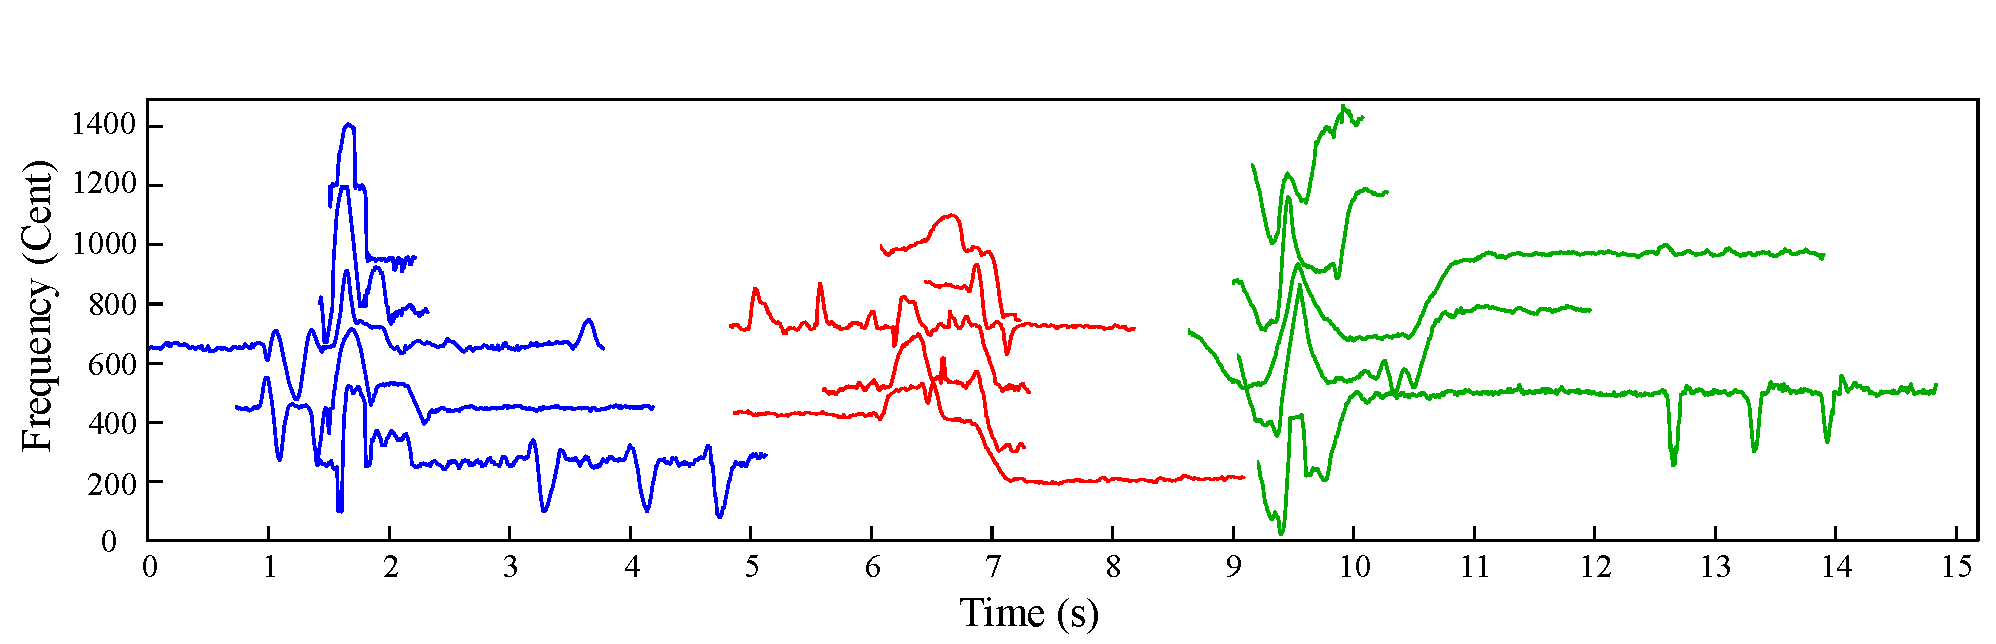
\includegraphics[width=\figSizeHundred]{ch01_introduction/figures/phraseClassesExample.pdf}
	\end{center}
	\caption{Pitch contours of occurrences of three different characteristic melodic phrases in Hindustani music. Contours are frequency transposed and time shifted for a better visualization.}
	\label{fig:phraseComplexityExample_intro}
\end{figure}

\textquote*[Cambouropoulos2006]{\textit{Music becomes intelligible to a great extent through self-reference, i.e.,~through the relations of new musical passages to previously heard material. Structural repetition and similarity are crucial devices in establishing such relations}}.

\textquote[schenker1980harmony]{Only by repetition can a series of tones be characterized as something definite. Only repetition can demarcate a series of tones and its purpose. Repetition thus is the basis of music as an art}. 

Analysis of repeating melodic patterns has been instrumental in the description of melodies by a large number of computational approaches in MIR. Repeating melodic patterns are integral to the melodic framework in IAM, the raga. They act as building blocks to construct melodies within the \gls{raga} grammar. Thus, IAM provides a context to develop computational approaches for discovery and characterization of melodic patterns from audio collections. However, improvisatory nature of this music tradition makes it a challenging task. The characteristic melodic phrases of \glspl{raga} act as the basis for artists to improvise, providing them with a medium to express creativity during \gls{raga} rendition. Artists bring in novelty through creatively transforming these melodic phrases as much as possible within the periphery defined by the \gls{raga} grammar. Therefore, the surface representation of these melodic phrases vary a lot across their occurrences. This high degree of variation in terms of the overall duration of a phrase, non-linear time warpings and the added melodic ornaments together pose a big challenge for melodic similarity computation and pattern extraction in \gls{iam}. In~\figref{phraseComplexityExample_intro} we illustrate this variability by showing the pitch contours of the different occurrences of three characteristic melodic phrases of the \gls{raga} Alaiya Bilawal. We can clearly see that the duration of a phrase across its occurrences varies a lot and the steady melodic regions are highly varied in terms of the duration and the presence of melodic ornaments. This characteristics of melodic patterns in IAM provide an opportunity to gain deeper insights into the perception of melodic similarity as well as how it is influenced by different cultural aspects. 


Computational complexity is often a primary concern in pattern discovery approaches. long duration of the performances in \gls{iam} pose a unique challenge. For the long duration audio recordings lasting around an hour discovering melodic patterns using music parallelism [Emilios] becomes a computationally challenging task.


\cite[p. 96]{martinez2001semiosis} (original definition given by Stern, 1933);

\blockquote{The \gls{raga} is more fixed than a mode, and less fixed than the melody, beyond the mode and short of melody, and richer both than a given mode or a given melody...}

This definition is closely related to the one given by~\cite{powers1963background};

\blockquote{A \gls{raga} is not a tune, nor is it a `modal' scale, but rather a continuum with scale and tune as its extremes.}

Raga thus is a fascinating topic of research. Being a complex framework it involves an intricate interplay between different melodic elements both in terms of the tonality and their temporal relations. Therefore, its computational characterization and recognition poses unique challenges as well as provides new opportunities. It is worth mentioning that recognizing raga in a musical performance requires domain expertize, which further emphasizes the complexity of the task.

Overall, we see that the main challenges in the computational melodic description of IAM arise due to its melodic complexity. It provides a context that is highly conducive to developing novel computational approaches to describe higher level melodic aspects of music, specifically of music performances in audio collections. 


\section{Scope and Objectives}
\label{sec:scope_objectives}


In this section we define the scope of our research work, clearly outline our objectives and enumerate the research questions addressed in this dissertation. 

Computational description and characterization of melodies is a broad research topic that can be approached from a number of perspectives involving different disciplines of science. In this dissertation we take a data-driven engineering approach and focus solely on the computational aspects of melodic analysis, building on top of established music theories. Our applied research methodology, stands at an intersection of signal processing, machine learning and time-series analysis. We focus on content-based processing and the input data used in our approaches comprise audio recordings. The only exception to this is the approach described in~\secref{sec:patterns_characterization_of_melodic_patterns}, which utilize the associated editorial metadata of the recordings in addition to the audio data. The approaches proposed in this thesis are devised and evaluated on music collections in \gls{iam} that includes both Hindustani and Carnatic music. We now outline our broad objectives in this dissertation.

\begin{itemize}
	\item To build a representative music corpora of \gls{iam} that comprises audio recordings and relevant editorial metadata, and use that to compile sizable and well annotated tests datasets for melodic analyses.
	\item To devise a data-driven computational approach to discover musically relevant melodic patterns in sizable audio collections of \gls{iam}
	\item To devise culture-aware and human interpretable approaches for automatic \gls{raga} recognition.
\end{itemize}


\TODO{enumerate all these tasks} There are a number of research tasks within computational melodic analysis that are addressed in this dissertation, which sum up to achieve our broad objectives. We list these tasks in~\figref{fig:tasks}, starting from the bottom and building to the top. We now provide a brief description of these specific tasks to show their relation and relevance in our broad objectives. 

\begin{figure}[h]
	\begin{center}
		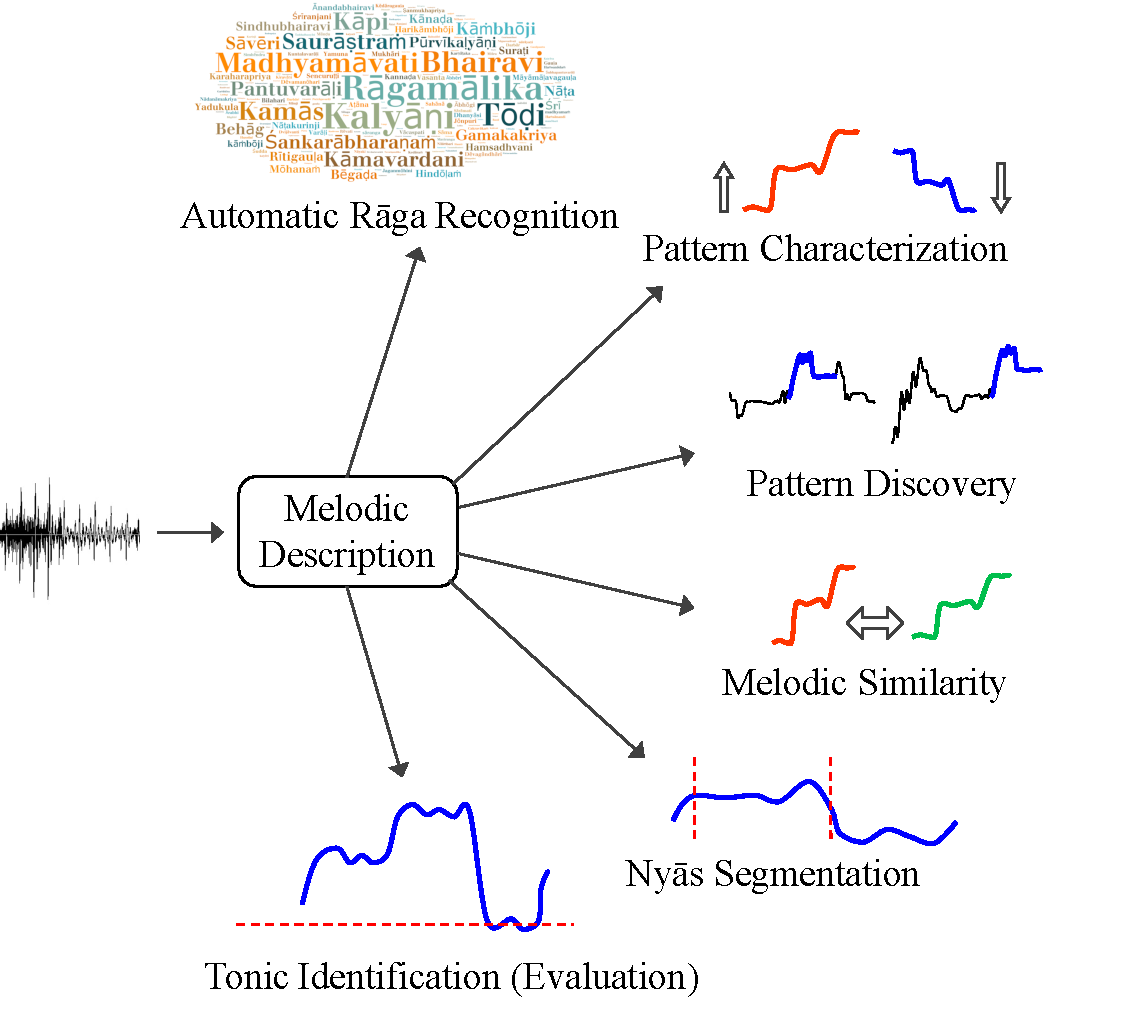
\includegraphics[width=\figSizeHundred]{ch01_introduction/figures/tasks.pdf}
	\end{center}
	\caption{Computational tasks within melodic analysis of \gls{iam} addressed in this dissertation.}
	\label{fig:tasks}
\end{figure}

As mentioned before, tonic pitch of the lead artist in a performance is the base frequency used for tuning by other instruments. For a meaningful comparison of melodies across artists and their recordings, identification of the tonic pitch in a recording is a fundamental task. In recent years a number of methods are proposed for tonic identification, however, there is no consensus on the best performing approach since the evaluations are performed on different datasets, under different experimental conditions. We address this issue by performing an extensive comparative evaluation of seven different tonic identification methods on six diverse datasets of \gls{iam} and identify the approaches that are robust and more accurate on both Hindustani and Carnatic music. In the process we also gain valuable insights into the types of errors made by tonic identification approaches, a useful information while devising methods that require tonic of the recordings as one of the inputs.

Melody segmentation is an important and a well researched topic in melody description in \gls{mir}. It is a crucial step in pattern processing tasks, specifically in the task of discovering melodic patterns. To the best of our knowledge, there are no computational approaches that directly address phrase segmentation in melodies of \gls{iam} from audio recordings\footnote{At the time of starting of this thesis work, 2012}. It is well known from musicological studies that \gls{nyas} \gls{svara} occurrences mark the boundaries of characteristic melodic phrases of \glspl{raga} in melodies of Hindustani music. Thus, detection of such segments in melodies can be an approach to melodic segmentation. We therefore address the task of automatically segmenting \gls{nyas} \gls{svara} segments in the melodies of Hindustani music. 

Musically meaningful computation of melodic similarity is one of the most crucial steps in melodic pattern extraction. Since the task of melodic pattern discovery follows an unsupervised approach, its quantitative evaluation on sizable music collections is a challenging task. As a result of which, evaluation of the methods used for computing melodic similarity also becomes difficult. Computation of melodic similarity in \gls{iam} is a work in progress and it has gained popularity during the course of this thesis. While addressing the task of computing melodic similarity in \gls{iam} we aim to clearly understand the challenges involved in the task, to analyze quantitatively the influence of different processing steps and parameter values on the accuracy, and to finally select the best possible method that can be used for the pattern discovery task. Our main intention behind investigating melodic similarity is to bootstrap our approach for melodic pattern discovery. 

We subsequently address the task of pattern discovery from large audio collections of \gls{iam}, which is one of the main objectives in this dissertation. In melodic pattern discovery we aim to extract all kinds of repeated melodic patterns, which can correspond to different types of melodic units in \gls{iam} with varying degree of musical relevance. In order to successfully use the discovered melodic patterns in analyzing high-level musical concepts such as \gls{raga}, it becomes important to assess the musical relevance of the discovered patterns. We therefore address the task of pattern characterization to identify the musically most relevant melodic patterns, the characteristic phrases of \glspl{raga}.

Finally, we investigate one of the most studied and relevant topics in computational anlaysis of \gls{iam}, automatic \gls{raga} recognition. We aim to devise a culturally-aware approach utilizing the main cues that listeners of \gls{iam} exploit to recognize \glspl{raga}. 

This work in this thesis is done as a part of the CompMusic project, and it aligns with the goals of the project. The objectives of this thesis are directed towards a bigger goal of developing culture-aware computational approaches that can utilize domain knowledge in order to produce semantically meaningful description of music. This thesis is also well aligned with the project's philosophy of open-access and reproducible research. All the data and code used to produce the results reported in this thesis is made openly available, with the exception of the commercial recordings, which is made accessible through personal contact\TODO{Ask xavier what to write!!}. In addition, whenever possible, we also make the output of our methods available to further facilitate reproducing the research results reported in this thesis.


\TODO{Should we be writing specific research questions???? given that our work is quite applied. Ask Xavier and Joan and then decide!!}

\section{Organization and Outline of the thesis}
\label{sec:organization_thesis}

\COMMENT{If time permits draw a block diagram of the different components in this thesis and we can arrange them chapter wise, that would look good and the navigation becomes easier}

There are eight chapters in this thesis. However, the primary contributions are contained in four chapters, Chapter\,3 to Chapter\,6. Each of these four chapters contain one main topic of this thesis, data corpus and datasets, data pre-processing procedures, melodic pattern processing and \gls{raga} recognition. A significant amount of the content in these chapters is derived from our peer-reviewed research papers~\cite{Gulati2014Tonic,gulati2014Landmark,gulati_SITIS_2014,gulati_ICASSP2015,gulati_ISMIR_2015,gulati_communities_2016,gulatiphrase_2016,gulati_tdms_2016}. Most of the work in these papers is done in collaboration with other researchers and musicians, which is duly indicated wherever required. We now proceed to describe a detailed outline of this thesis.

In \chapref{chap:background}, we provide an overview of the music and scientific background and review relevant literature available on the topics addressed in this thesis. We begin with a short description of the terminology used in this thesis. We then provide a brief introduction to \gls{iam} and of the music concepts directly related to melodic aspects in this music tradition. We review existing research within \gls{mir} that relate to the topics covered in this dissertation. We analyze separately the literature that focuses on computational analysis of \gls{iam} and the one for other music traditions of the world. We finally present an overview of the relevant scientific background needed to better understand the technical concepts discussed in this thesis. Our main contribution in this chapter is in reviewing the relevant literature and compiling it.

In \chapref{chap:corpus_music_corpora_and_datasets}, we present an overview of the music corpora and test datasets of \gls{iam} that are compiled as a part of the CompMusic project. We enumerate the set of design criterion followed to build music corpora for research in \gls{iam}~\citep{serra:14:corpus}. We describe both Hindustani and Carnatic music corpus and present a short evaluation of the goodness of the corpora with respect to different criterion. Subsequently, a detailed description of the individual test datasets used for evaluations in this thesis is provided. The content of this chapter is derived from~\citep{serra:14:corpus,CM_Corpora_Ajay14}. Our main contributions in this chapter are in building the research corpora, which was a team effort, and compiling and annotating different test datasets with the help from musicians.

In \chapref{chap:data_preprocessing}, we describe different data pre-processing blocks employed in our work to obtain musically relevant melody representations and descriptors that will be used by the methods described in the subsequent chapters. The main goal in this chapter is to present an extensive comparative evaluation of the available tonic identification approaches to select the best approach that will be used in this work, and to present our novel method for \gls{nyas} segmentation in melodies of \gls{iam}. These two tasks primarily cover our novel contributions in this chapter. In addition, we also present an overview of the methods that we use to obtain a melody representation from audio recordings.

In \chapref{chap:melodic_pattern_processing}, we present our main contributions in melodic pattern processing in \gls{iam}. There are three related topics discussed in this chapter, melodic similarity, pattern discovery and pattern characterization. We first investigate relevant melodic similarity measures with an objective to learn the influence of different choices of melody representation, distance measure and normalization strategy on melodic similarity computation for characteristic melodic patterns of \glspl{raga}. In the process we propose a novel approach to improve melodic similarity by exploiting specific characteristics of melodies in \gls{iam}. Having learned the optimal set of procedures and system parameters in an supervised setup, we utilize this knowledge for discovering melodic patterns in audio collections of \gls{iam}, in which we follow an unsupervised methodology. Finally, we discuss a novel approach to characterize the discovered melodic patterns in order to identify the ones that correspond to \gls{raga} motifs. All four studies reported in this chapter are based on our novel contributions.

In \chapref{chap:raga_recognition}, we present the other significant part of our scientific contributions in the thesis. This chapter addresses one of the most studied topics in computational analyses of \gls{iam}, automatic \gls{raga} recognition. We propose two novel approaches for \gls{raga} recognition. Our first approach utilizes melodic patterns, which are the most prominent cues for \gls{raga} recognition used by the human listeners. We utilize the discovered melodic patterns from previous chapter and employ vector space modeling techniques to model \glspl{raga}. In our second approach we propose a novel melodic representation inspired by the concept of delay coordinates. This representation encodes both the tonal and the temporal aspects of melodies that are relevant to characterize \glspl{raga}. We perform comparative evaluations with the existing methods and show that our system outperforms state of the art by significant margins.

In \chapref{sec:applicatoins}, we present applications and a demo that are based on the research outcomes in CompMusic, which also includes the work done in this thesis. In particular, we introduce Dunya, a web-based research prototype that exposes the resarch outcomes and resources in the CompMusic project and consolidates the tools and technology developed in the project. We provide a brief description of both the interfaces, web-interface and web-API, that Dunya offers to access the content. In addition, we introduce two real-world applications; Saraga and Riyaz, that capitalize on our research outcomes in CompMusic and cater to two types of use-cases, enhance listening and music education. In order to demonstrate the outcome of our melodic pattern processing approaches more directly, we also present a web-based demo. It shows a network-based navigation across discovered melodic patterns and audio recordings. \TODO{written very roughly change it after you have more idea of that chapter}

At the end of every chapter listed above we present a summary of the results and conclusions. Finally, in \chapref{sec:conclusoins} we present the overall conclusions of this thesis work, list our main contributions and discuss possible future directions for improving melodic description of \gls{iam}. This thesis also contains three appendix sections. Appendix A, lists the publications by the author, Appendix B, present ways to access the relevant resources and Appendix C, presents the glossary of the abbreviations and other terms used in this thesis.


